\documentclass{article}\usepackage[]{graphicx}\usepackage[]{xcolor}
% maxwidth is the original width if it is less than linewidth
% otherwise use linewidth (to make sure the graphics do not exceed the margin)
\makeatletter
\def\maxwidth{ %
  \ifdim\Gin@nat@width>\linewidth
    \linewidth
  \else
    \Gin@nat@width
  \fi
}
\makeatother

\definecolor{fgcolor}{rgb}{0.345, 0.345, 0.345}
\newcommand{\hlnum}[1]{\textcolor[rgb]{0.686,0.059,0.569}{#1}}%
\newcommand{\hlstr}[1]{\textcolor[rgb]{0.192,0.494,0.8}{#1}}%
\newcommand{\hlcom}[1]{\textcolor[rgb]{0.678,0.584,0.686}{\textit{#1}}}%
\newcommand{\hlopt}[1]{\textcolor[rgb]{0,0,0}{#1}}%
\newcommand{\hlstd}[1]{\textcolor[rgb]{0.345,0.345,0.345}{#1}}%
\newcommand{\hlkwa}[1]{\textcolor[rgb]{0.161,0.373,0.58}{\textbf{#1}}}%
\newcommand{\hlkwb}[1]{\textcolor[rgb]{0.69,0.353,0.396}{#1}}%
\newcommand{\hlkwc}[1]{\textcolor[rgb]{0.333,0.667,0.333}{#1}}%
\newcommand{\hlkwd}[1]{\textcolor[rgb]{0.737,0.353,0.396}{\textbf{#1}}}%
\let\hlipl\hlkwb

\usepackage{framed}
\makeatletter
\newenvironment{kframe}{%
 \def\at@end@of@kframe{}%
 \ifinner\ifhmode%
  \def\at@end@of@kframe{\end{minipage}}%
  \begin{minipage}{\columnwidth}%
 \fi\fi%
 \def\FrameCommand##1{\hskip\@totalleftmargin \hskip-\fboxsep
 \colorbox{shadecolor}{##1}\hskip-\fboxsep
     % There is no \\@totalrightmargin, so:
     \hskip-\linewidth \hskip-\@totalleftmargin \hskip\columnwidth}%
 \MakeFramed {\advance\hsize-\width
   \@totalleftmargin\z@ \linewidth\hsize
   \@setminipage}}%
 {\par\unskip\endMakeFramed%
 \at@end@of@kframe}
\makeatother

\definecolor{shadecolor}{rgb}{.97, .97, .97}
\definecolor{messagecolor}{rgb}{0, 0, 0}
\definecolor{warningcolor}{rgb}{1, 0, 1}
\definecolor{errorcolor}{rgb}{1, 0, 0}
\newenvironment{knitrout}{}{} % an empty environment to be redefined in TeX

\usepackage{alltt}
\IfFileExists{upquote.sty}{\usepackage{upquote}}{}
\begin{document}

\begin{knitrout}
\definecolor{shadecolor}{rgb}{0.969, 0.969, 0.969}\color{fgcolor}\begin{kframe}


{\ttfamily\noindent\itshape\color{messagecolor}{\#\# Registered S3 method overwritten by 'quantmod':\\\#\# \ \ method \ \ \ \ \ \ \ \ \ \ \ from\\\#\# \ \ as.zoo.data.frame zoo}}\end{kframe}
\end{knitrout}

\section*{Line Charts and Time Series Visualization}

A \textbf{Line chart}, often referred to as a line graph or line plot, is a statistical chart composed of a Cartesian coordinate system, some points, and lines. It is commonly used to represent changes in numerical values over continuous time intervals or ordered categories. In a line graph, the x-axis is typically used for continuous time intervals or ordered categories (such as Stage 1, Stage 2, Stage 3). The y-axis is used for quantified data, and if it is negative, it is plotted below the y-axis. Lines are used to connect adjacent data points.

Line graphs are used to analyze trends in things that change over time or ordered categories. If there are multiple sets of data, they are used to analyze the interaction and impact of these data sets over time or ordered categories. The direction of the line represents positive/negative changes, and the slope of the line indicates the degree of change.

In terms of data, a line graph requires a continuous time field or a categorical field and at least one continuous data field.


\subsection{Basic Components}
\begin{itemize}
  \item \textbf{X-Axis (Horizontal Axis):} Typically represents the independent variable, such as time or date.
  \item \textbf{Y-Axis (Vertical Axis):} Typically represents the dependent variable, like sales numbers, stock prices, or temperatures.
  \item \textbf{Line:} Connects the individual data points. In some line charts, multiple lines can represent different categories or sets of data.
\end{itemize}


\subsection{Suitability for Displaying Trends Over Time:}
\begin{itemize}
    \item \textbf{Visual Clarity:} Line charts provide a clear and concise way to view changes over time. When data points are plotted over regular intervals (e.g., days, months, years), it becomes easy to see upward or downward trends.
    \item \textbf{Comparisons:} When you have multiple lines on a single chart, you can easily compare different sets of data. For instance, comparing sales data of two different products over time.
    \item \textbf{Identification of Patterns:} Line charts help in identifying patterns and anomalies. Seasonal patterns, cyclical events, and unexpected spikes or dips become evident.
    \item \textbf{Forecasting:} By viewing historical data trends on a line chart, analysts can make predictions or forecasts for future data points.
    \item \textbf{Simplicity:} They are easy to understand and interpret. Even if someone isn't data-savvy, they can grasp the general trend and major fluctuations from a line chart.
    \item \textbf{Flexibility:} They can be used for both short-term and long-term data. Whether you're looking at stock prices minute-by-minute over a single day or global temperature averages over a century, line charts can effectively represent the data.
\end{itemize}


\subsection{Limitations:}
While line charts are excellent for displaying trends over time, they have limitations. They may not be suitable for showing individual data distributions or for data where there's no logical order. eg. too many points, too many lines, too many zeros.\\


\subsection*{Discuss the importance of time series visualisation in data analysis.}

Time series visualization refers to the graphical representation of time-ordered data points. In the world of data analysis, this form of visualization is invaluable for examining patterns, anomalies, and trends in datasets that evolve over time.\\
\textbf{Uncovering Trends:}\\
One of the primary advantages of time series visualization is the ease with which it allows analysts to identify long-term upward or downward trends in data. Recognizing these trends can help organizations make informed decisions about future strategies or interventions.\\
\textbf{Detection of Seasonality:}\\
Many datasets exhibit patterns that repeat over specific intervals, such as days, months, or years. Time series visualization makes it straightforward to spot such cyclical behaviors, which can be vital for businesses in sectors like retail or agriculture.\\
\textbf{Identifying Anomalies:}\\
Graphical representations can quickly highlight data points or periods that deviate significantly from the norm. These anomalies can indicate errors in data collection, or they may reveal significant events that need to be further investigated.\\
\textbf{Forecasting and Predictions:}\\
After identifying patterns in historical data, time series visualizations can aid in modeling future data points. Predictive modeling, underpinned by clear visualizations, allows businesses to make proactive decisions.\\
\textbf{Facilitating Comparative Analysis:}\\
Time series charts often allow for overlaying multiple data series on a single graph. This capability is useful for comparing different datasets or the same dataset under different conditions, leading to more comprehensive insights.\\
\textbf{Conclusion:}\\
Time series visualization is an indispensable tool in the arsenal of data analysts. It condenses large volumes of chronological data into easily interpretable graphics, enabling quick insights, better decision-making, and a deeper understanding of temporal dynamics in datasets. By providing a clear view of data trends, seasonality, and anomalies, time series visualization facilitates more informed and strategic actions in various domains.



\section*{Provide best practices for creating clear and informative line charts.}

\begin{itemize}
  \item Title and Labels: Every chart should have a descriptive title and axis labels to clearly convey the purpose of the visualization and the data being shown.
  \item Use of Colors: Colors should be chosen to clearly differentiate between different lines or data points but also be consistent with the overall theme or style.
  \item Gridlines and Background: Soft gridlines can help the viewer estimate values. A clean background aids in clarity.
  \item Line Types and Point Shapes: When multiple lines are on the same chart, use different line types and point shapes to differentiate between them.
  \item Consistent Scaling: The scale on the y-axis should be consistent so that the viewer isn't misled.
  \item Annotations: Important points or changes can be annotated directly on the graph.
  \item Legends: If there are multiple lines or data points with different colors/shapes, a legend should be provided.
\end{itemize}

Let's apply these practices:

First, we generate 2 series of random data.

\begin{knitrout}
\definecolor{shadecolor}{rgb}{0.969, 0.969, 0.969}\color{fgcolor}\begin{kframe}
\begin{alltt}
\hlstd{x} \hlkwb{<-} \hlkwd{seq}\hlstd{(}\hlnum{1}\hlstd{,} \hlnum{20}\hlstd{)}
\hlstd{y} \hlkwb{<-} \hlkwd{runif}\hlstd{(}\hlnum{20}\hlstd{)}
\hlstd{data} \hlkwb{<-} \hlkwd{data.frame}\hlstd{(}\hlkwc{x} \hlstd{= x,} \hlkwc{y} \hlstd{= y)}
\end{alltt}
\end{kframe}
\end{knitrout}

Below is a line chart of the random sample:

\begin{knitrout}
\definecolor{shadecolor}{rgb}{0.969, 0.969, 0.969}\color{fgcolor}
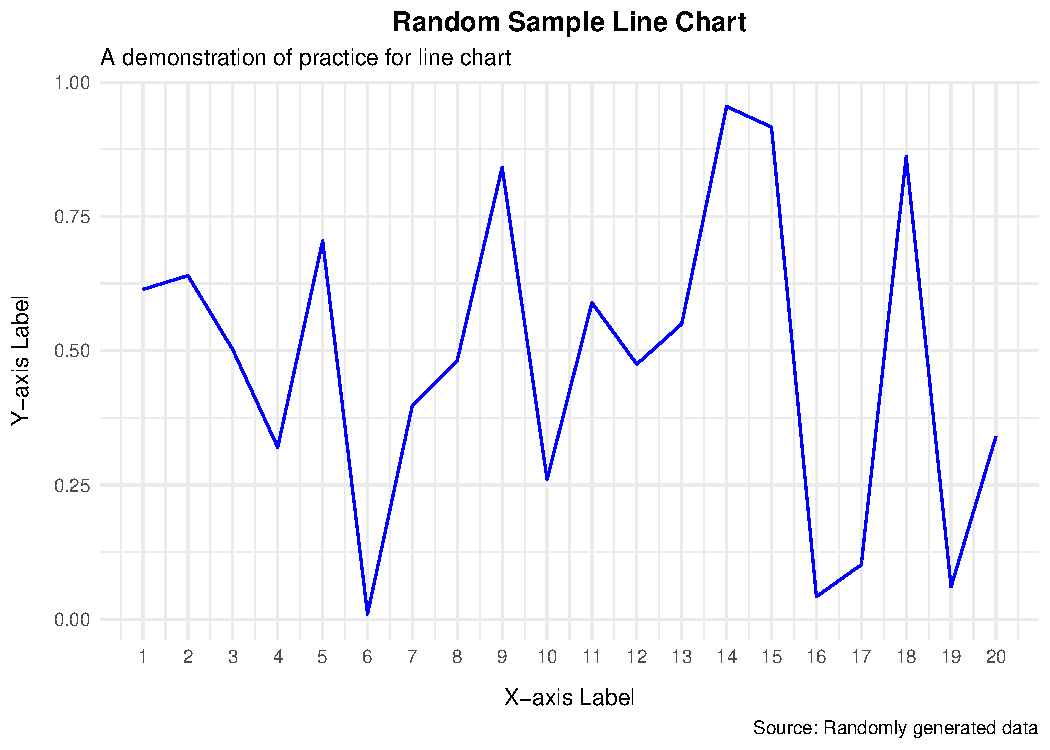
\includegraphics[width=\maxwidth]{figure/plot-chunk-1} 
\end{knitrout}


\section*{Showcase real-world examples of time series visualisations.}

Time series of the daily CNY, CAN, EUR, HKD, USD versus GBP exchange reference rate data
published by the European Central Bank over the time period from 01 Jan 2013 to 12 Oct 2023 (without weekends). The exchange rate tells you how many pounds you need to buy/sell 1 CNY, CAN, EUR, HKD, USD.

\subsection{The data set has the format as below:}

\begin{table}[h]
\centering
\begin{tabular}{|c|c|c|c|c|c|}
\hline
\textbf{Date} & \textbf{CNYtoGBP} & \textbf{CANtoGBP} & \textbf{EURtoGBP} & \textbf{HKDtoGBP} & \textbf{USDtoGBP} \\
\hline
\%d-\%m-\%y & Value & Value & Value & Value & Value \\
\hline
& & & & & \\
\hline
\end{tabular}
\caption{Field Information: CNY, CAN, EUR, HKD, USD to GBP}
\end{table}


\subsection{Multiple time series in one plot:}

\begin{knitrout}
\definecolor{shadecolor}{rgb}{0.969, 0.969, 0.969}\color{fgcolor}
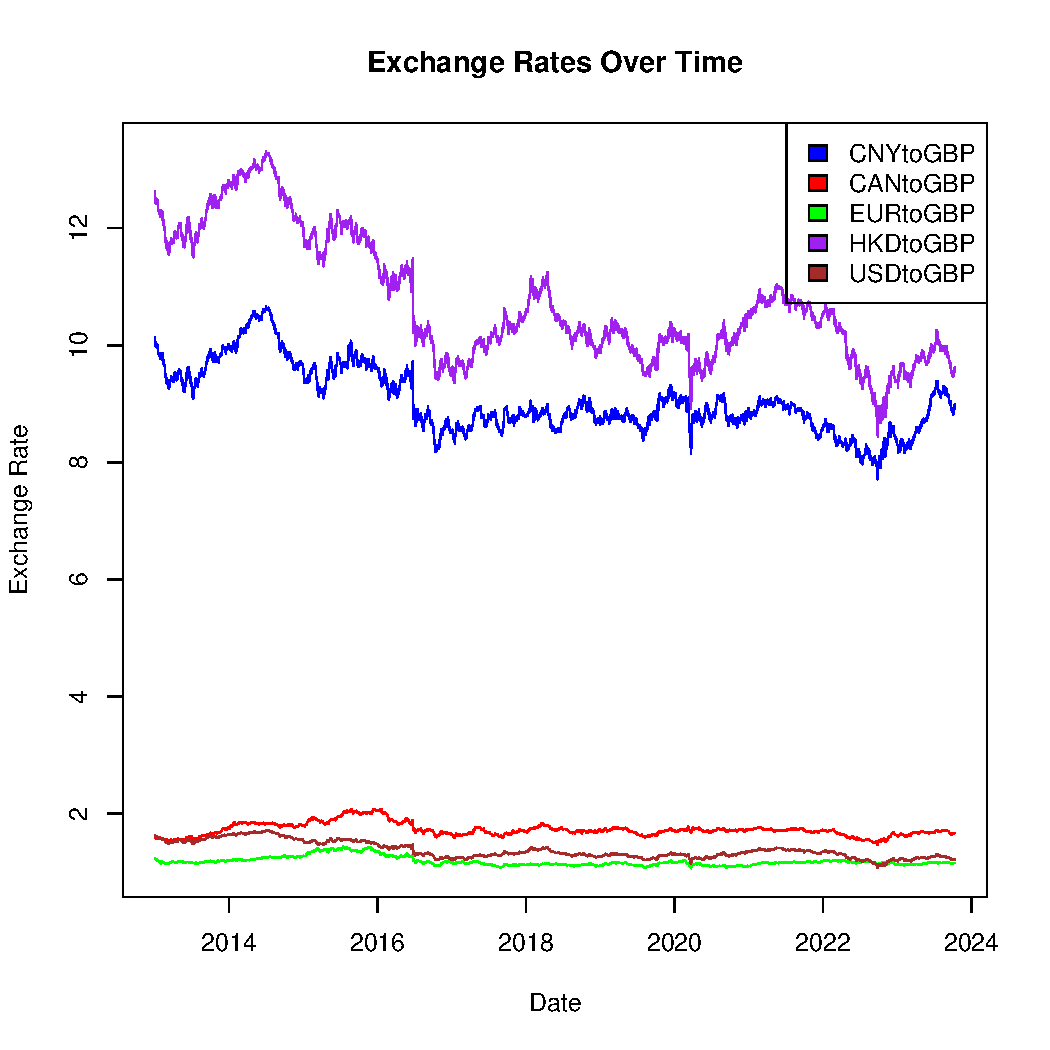
\includegraphics[width=\maxwidth]{figure/unnamed-chunk-1-1} 
\end{knitrout}

\subsection{Decomposition of one time series into trend, seasonal, and random.}


One of the primary advantages of time series visualization is the ease with which it allows analysts to identify long-term upward or downward trends in data and patterns that repeat over specific intervals. By decomposing the time series, it would be easy to see those features.

\begin{knitrout}
\definecolor{shadecolor}{rgb}{0.969, 0.969, 0.969}\color{fgcolor}
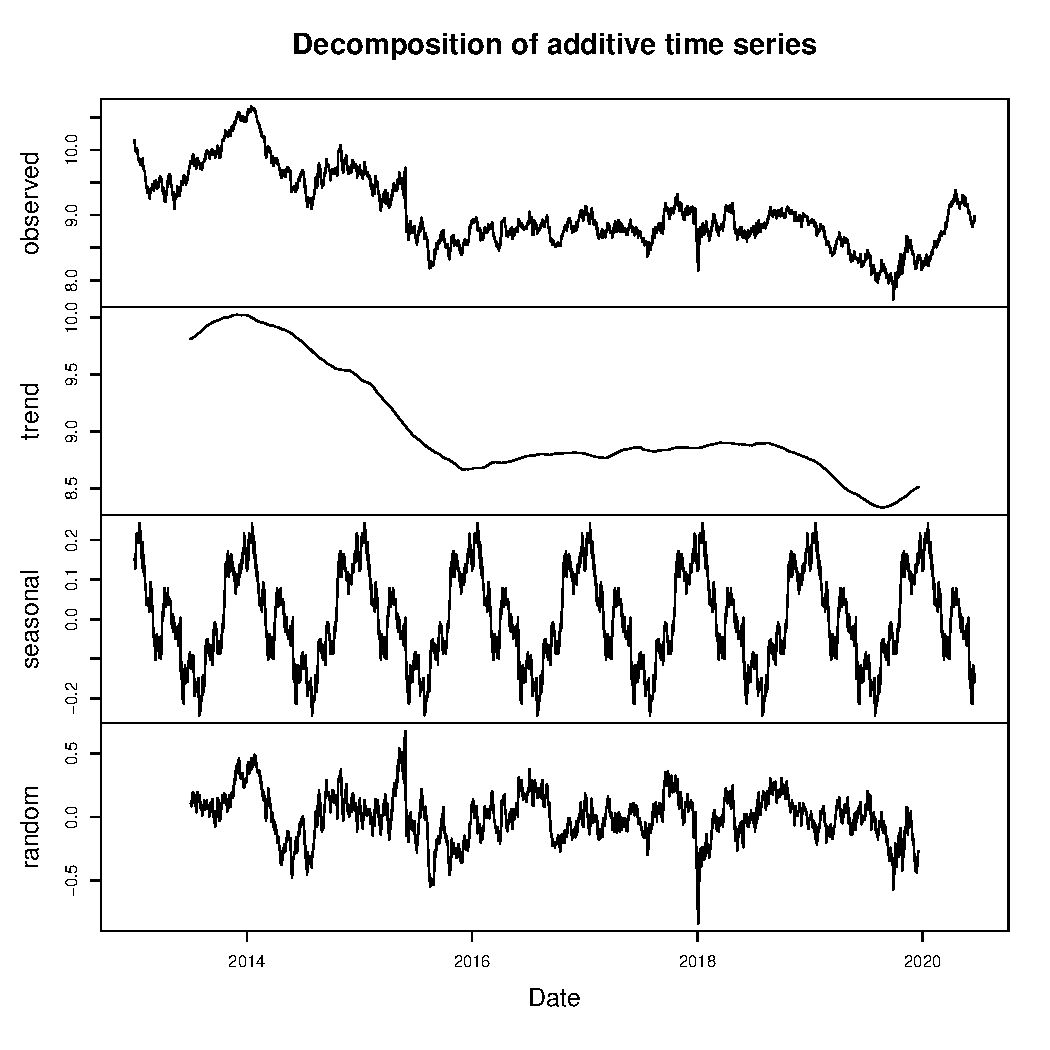
\includegraphics[width=\maxwidth]{figure/unnamed-chunk-2-1} 
\end{knitrout}


\subsection{Double y-axis time series plot.}

If we want to display two different time series that measure two different quantities at the same time points, we can draw the second series again on the second Y-axis on the right side.

\begin{knitrout}
\definecolor{shadecolor}{rgb}{0.969, 0.969, 0.969}\color{fgcolor}
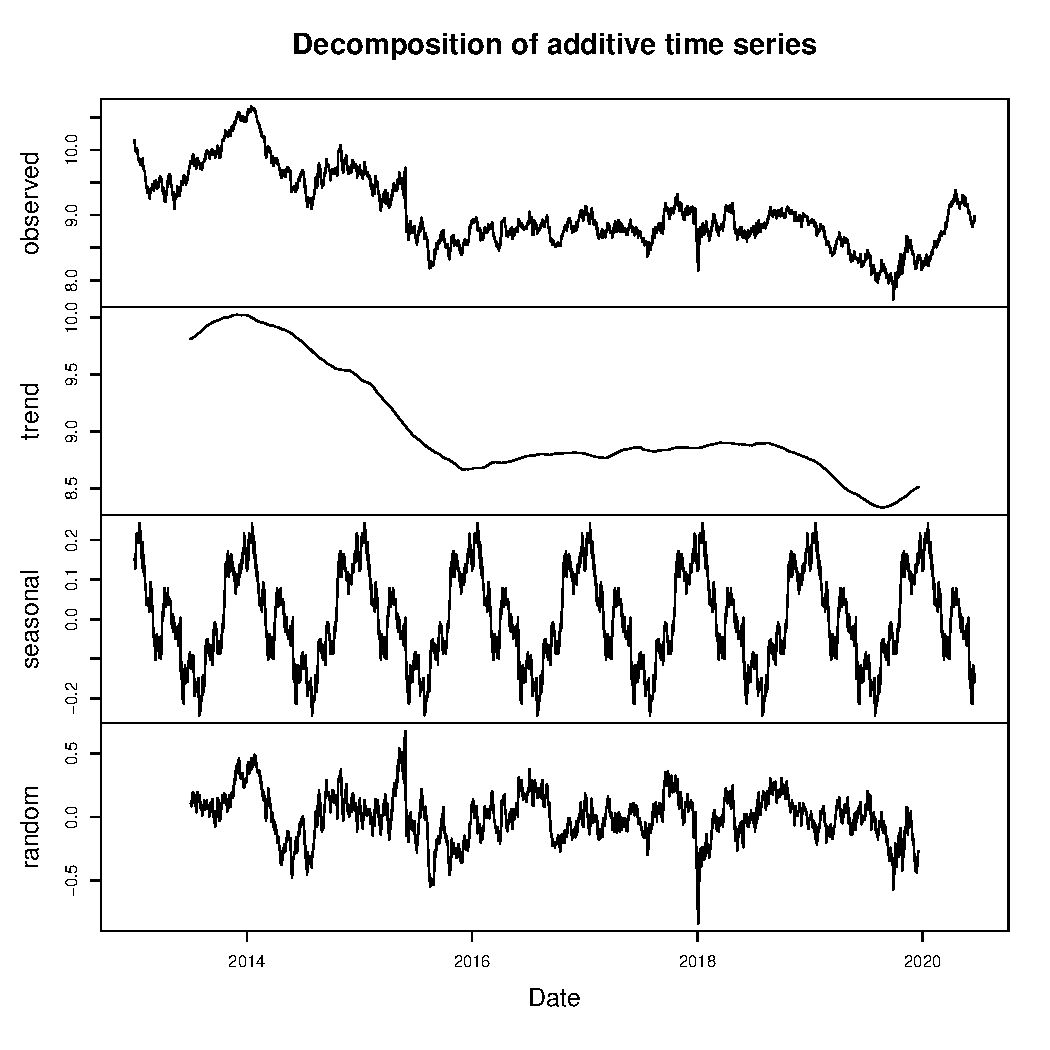
\includegraphics[width=\maxwidth]{figure/unnamed-chunk-3-1} 
\end{knitrout}




\end{document}
